% - Weak Scalability Design : Keep Pipeline of Ensembles to show barrier
%   needed in S5 and S6.
% - Performance, generality with weak scaling (agnostic to kernel) Added
%   functionality (do not speak about binding adaptivity to performance or
%   generality).
% - In use case: add in why TIES is challenging, and why adaptivity is
%   challenging.

\mtnote{General note. \\
        - Currently, this section is a merge of two distinct contributions.
          These need to be better merged. For example, we should consider
          whether (i) the description of the adaptive experiments should be
          moved to the first subsection ``Experimental Setup''; (ii) Table 1
          should be extended to include the adaptive/nonadaptive properties;
          (iii) the discussion of the results should have a uniform
          argumentative format; etc.\\
        - The structure of the section should be revise making the division
          in subsections consistent and changing/refining their naming.\\
        - A.0,1,2 require major rewriting of the text and the writing of
          relevant portions of new text. This includes: (i) eliminating
          redundant (copied) text; (ii) Eliminating or referencing text
          copied from other publications; (iii) reorganize the argumentation
          following the other general note left in the comments and better
          separating the experimental variables (especially including
          adaptive/nonadaptive) properties; (iv) adding plots (even if with
          incomplete results) and writing an actual analysis of the results
          for each plot.}


\jdnote{Revisions: \\ 
        - Rewrote experimental setup by starting with motivation and explaining
          overview of experiments
        - Appended all experiments to table
        - Created subsections for weak scaling, strong scaling, validation, 
          adaptive experiments
        - Added plots (some are incomplete) and rearranged analysis
        - Kristof added his data on (06/03) for adaptive experiments and wrote 
        results (adaptive plots to come Tuesday 06/05)
        - Strong scaling subsection still needs to be addressed}
% ---------------------------------------------------------------------------
\subsection{Experiment Setup}\label{ssec:exp_design}

Computational drug campaigns require sizable compute resources in order to 
run concurrent simulations for a large number of drug candidates. Therefore, 
we perform our experiments on machines that can deliver at the scale necessary 
to support these demands. \jdnote{should we mention anything about exascale?}
Before embarking on such drug campaign which utilize 150 million core hours
(award) on NCSA Blue Waters, we perform experiments to characterize the 
overheads of HTBAC, its runtime system and the weak and strong scaling 
performance on Blue Waters. We validate our free energy calculation results 
produced using HTBAC with results previously cited not having used HTBAC. 

Given that certain protocols such as TIES are more computationally demanding, 
the efficient use of resources becomes paramount, especially for campaigns that 
are limited by a computational budget. Compared to non-adaptive 
methods, adaptive methods as described in Section III and Section IV are able to 
reduce the number of simulations for each lead candidate and thereby reduce
computational load, without a loss in free energy accuracy. Adaptive methods 
can support a type of computational efficiency by improving the rate of 
statistical convergence given a defined number of resources. This requires 
a framework like HTBAC that can support runtime decisions to redistribute 
resources in order support new simulations based on intermediate results. Using 
HTBAC, we perform adaptive experiments that require such runtime decisions and 
compare and characterize resource efficiency with non-adaptive experiments. 


% Commented section below will go in Section III and Section IV

% -------------------------------------------------------------------------- %

% Drug screening typically occurs in two phases. The first phase runs simulations 
% of all drug candidates and determines which candidates become lead candidates. 
% This phase is performed using less computationally intensive protocols such as 
% ESMACS. Once we eliminate poor-binding candidates, we begin the second phase of 
% the campaign where we investigate lead compounds using computationally more 
% demanding protocols such as TIES. During the second phase, the accuracy of each 
% candidate is evaluated. A high level of variability exists in the chemical 
% properties across candidates. Therefore, the TIES protocols assumes the most 
% general case in evaluating the binding free energy accuracy. To maintain 
% generality, the TIES protocol requires 13 evenly spaced simulations, captured 
% using a sampling parameter references as $\lambda$ windows in Section III. 
% Although generality asserts the correct convergence criteria, this approximation 
% of $\lambda$ windows induces higher computational costs as a result of executing 
% large yet sometimes unnecessary simulations. 

% On the other hand, adaptive methods such as the adaptive quadratures  
% highlighted Section III, require less 
% sampling and thereby reduce the number of simulations, without sacrificing 
% accuracy. Because this method is tailored to every candidate, there is no way
% to understand \textit{a priori} the placement of $\lambda$ windows and thereby 
% the total number of simulations. 

% This requires the ability to instantiate simulations that predicate on 
% intermediate results during runtime. 

% Define parameters: added simulations means task count adaptivity and
% task attribute adaptivity. The next set (both number of resources) of simulations 
% depends on the output properties of the previous simulations. When we adapt the 
% number of simulations, the distribution of resources for each task within a 
% static pilot will fluctuate. 

% Carefully constructed $\lambda$ placement requires that the workflow can be 
% adaptable by creating new computational tasks during execution, thereby modify 
% the task graph during runtime. In HTBAC, construction of an adaptive workflow
% is predicated upon the workload management system (define) that provides 
% expression of adaptive features. 

% while communicating those parameters down to the runtime system 
% (define).  


% The post-execution properties are captured by the workload management system,
% EnTK.


% We then perform adaptive experiments to show 
% improvements in time-to-convergence. 

% -------------------------------------------------------------------------- %


\begin{table*}
    \caption{Parameters of scalability and adaptivity experiments.}
    \label{tab:experiments}
    \centering
    \resizebox{\textwidth}{!}{
    \begin{tabular}{l            % Experiment ID
                    l            % experiment type
                    l            % physical system 
                    l            % CI
                    l            % protocol type
                    l            % number of protocols
                    l            % total cores
                    }
    %
    \toprule
    %
    \B{ID}                            &  % Experiment ID
    \B{Type of Experiment} &            % Adaptive or Scale
    \B{Physical System(s)} &            % Adaptive or Scale
    \B{Computing Infrastructure (CI)} &  % CI
    \B{Protocol(s)}                   &  % protocol type
    \B{No. Protocol(s)}                    &  % number of protocols
    \B{Total Cores}                     \\ % total cores
    % \B{Executable}                          \\ % executable
    %
    \midrule
    %
    \B{1}                             &  % Experiment ID
    Weak scaling                      &
    BRD4                              &
    Blue Waters                       &  % CI
    ESMACS                            &  % protocol type
    (2, 4, 8, 16)                     &  % number of protocols
    1600, 3200, 6400                  \\  % total cores
    % NAMD-MPI                               \\ % executable
    %
    % \B{2}                             &  % Experiment ID
    % Weak scaling                      &
    % BRD4                              &
    % Titan                          &  % CI
    % ESMACS                          &  % protocol type
    % (16, 64, 128)                    &  % number of protocols
    % 6400, 25600, 51200              &  % total cores
    % NAMD (non-MPI)                 \\ % executable
    % 
    \B{2}                             &  % Experiment ID
    Weak scaling                      &
    BRD4                              &
    Blue Waters                       &  % CI
    TIES                              &  % protocol type
    (2, 4, 8)                         &  % number of protocols
    4160, 8320, 16640                 \\  % total cores
    % NAMD-MPI                              \\ % executable
    % %
    % \B{4}                             &  % Experiment ID
    % Weak scaling                      &
    % BRD4                              &
    % Titan                          &  % CI
    % TIES                          &  % protocol type
    % (8, 32, 64)                    &  % number of protocols
    % 16640, 66560, 133120              &  % total cores
    % NAMD (non-MPI)                 \\ % executable
    %
    \B{3}                             &  % Experiment ID
    Weak scaling                      &
    BRD4                              &
    Blue Waters                       &  % CI
    ESMACS + TIES                     &  % protocol type
    (2, 4, 8)                    &  % number of protocols
    5280, 10560, 21120               \\ % total cores
    % NAMD-MPI                              \\ % executable
    %
    \B{4}                             &  % Experiment ID
    Strong scaling                      &
    BRD4                              &
    Blue Waters                          &  % CI
    TIES                          &  % protocol type
    (8, 8, 8)                    &  % number of protocols
    16640, 8320, 4160               \\ % total cores
    % NAMD-MPI                              \\ % executable
    %
    \B{5}                             &  % Experiment ID
    Strong scaling                          &  % CI
    BRD4                      &
    Blue Waters                              &
    ESMACS                          &  % protocol type
    (16, 16, 16)                    &  % number of protocols
    6400, 3200, 1600                \\ % total cores
    % NAMD-MPI                              \\ % executable
    %
    \B{6}                             &  % Experiment ID
    Non-adaptivity                       &  
    PTP1B, MC1, TYK2                     &  
    Blue Waters                          &  % CI                            
    TIES                          &  % protocol type
    (1, 1, 1)                           &  % number of protocols
    2080                           \\ % total cores
    %
    \B{7}                             &  % Experiment ID
    Adaptivity                       &  
    PTP1B, MC1, TYK2                  &  
    Blue Waters                          &  % CI                            
    TIES                          &  % protocol type
    (1, 1, 1)                           &  % number of protocols
    2080                           \\ % total cores
    % NAMD-MPI                              \\ % executable
    %
    \bottomrule
    %
    \end{tabular}
    }
\up{}
\end{table*}

    We show homogeneous and heterogeneous weak scalability of the protocols by
increasing the number of protocol instances while keeping the required number
of pipelines. By design of each protocol, an increase in the number of
instances means an increase in the number of pipelines. \jdnote{mention the 
relationship between protocols and pipelines in section IV.} By design of weak 
scaling, the ratio between the number of pipelines and cores are kept constant. 
As the number of cores (measure of resource) changes by a factor of 2, we 
introduce twice as many protocol instances. In this way, weak scaling provides 
insight into the size of the workload that can be investigated in a given amount 
of time.
% \mtnote{property
% of? I would replace with: ``weak scaling provides insight\ldots''} provides
% insight 
    Experiment 1 measures the weak scalability of HTBAC, EnTK and RP using 
multiple instances of the ESMACS protocols. Experiment 2 measures weak scaling 
performance of TIES. Experiments 3 repeats the same design as experiments 1 and 
2 using both TIES and ESMACS, to demonstrate heterogeneous protocol execution. 
% Experiment 2 measures weak scaling
% performance of ESMACS at higher scales, using ORNL Titan.
\mtnote{Would it be better to describe weak scaling in terms of solution
time, number of resources and problem size, as done in the following
paragraph?}\jdnote{moved to previous para when first introducing weak scaling}

    Next, we demonstrate strong scaling performance of the protocols by fixing 
the workload i.e. the number of pipelines but reducing the number of cores 
by a factor of 2 in each run. We measure how the timing of the workload scales 
when adding resources, \jdnote{expecting linear speedup, and expect fixed 
overheads} as well as the overheads in HTBAC, EnTK and RP. Experiments 4 
measures the strong scaling performance of ESMACS while experiment 5 repeats the 
same strong scaling experiment using the TIES protocol. 

    Lastly, we perform nonadaptive and adaptive experiments using the TIES 
protocol to demonstrate intra-protocol adaptivity \jdnote{define intra-protocol 
adaptivity in section IV}. 

% Keep iterating on the next two paragraphs to get the right description from
% Kristof 
% -------------------------------------------------------------------------- %
In the non-adaptive workflow, we use 13 pre-assigned and approximated $\lambda$ 
windows.  By design of the TIES protocol, each $\lambda$ 
window creates a new simulation condition that must be replicated. TIES requires 
5 replicas per $\lambda$, thereby producing $\lambda$ $4\times 5$
total simulations. \jdnote{Section IV will explain how
simulations map to computational tasks}. As described in the TIES workflow 
Figure \jdnote{include nonadaptive workflow}, this produces a total of 65 
concurrent simulations for stages $S1$ -- $S4$. The production simulation stage 
$S4$ executes each simulation for 4 nanoseconds (ns). The analysis stage, $S5$, 
assigns 5 analysis tasks which aggregate simulation results of $S4$ with 
respect to each replica. The global analysis stage $S6$ contains a single task
that aggregates the results from $S5$.  

In the adaptive workflow~\ref{fig:adaptive_ties}, we run shorter 1 ns MD 
production simulations, followed by a different analysis which estimates free 
energy errors with respect to each interval of two $\lambda$ values. The 
estimation of the error determines whether or not to spawn additional $\lambda$ 
windows. If the error estimate in a certain interval is higher than the 
acceptable threshold, a new $\lambda$ window is assigned halfway between the 
interval. If the critical threshold is reached, we have reached convergence and 
the application stops; else, current simulations continue executing and new 
simulations begin executing based on newly generated $\lambda$ windows. 

The estimation computation is captured as a single stage containing a single 
task. By design of the adaptive quadrature algorithm, the number of additional
$\lambda$ windows will vary across candidates, which will impact the number of simulation-analysis iterations. \jdnote{will call this something else}. 
\jdnote{check with Kristof on the local and global analysis that happen for 
nonadaptive}



% This procedure is
% repeated until convergence, at which point all concurrent simulation are
% terminated. We define convergence as the point in the production-analysis
% loop at which a desired error threshold is reached.


% move this to HTBAC Design & Implementation 
% -------------------------------------------------------------------------- %

% As discussed earlier, the free energy is calculated numerically using an integration algorithm, integrating the function $\partial U/\partial\lambda$ evaluated at discrete of $\lambda$. In a non-adaptive case these values of $\lambda$are selected a priori, and having no knowledge of the function's shape, equally spaced values are the optimal option. 



% The aim of the general adaptive quadrature algorithm is to minimize the number 
% of function evaluations while still estimating the integral under a specified 
% error threshold. In our case a function evaluation means the full simulation for 
% a given $\lambda$ window, and reducing this means a substantial efficiency gain. 


% where each stage runs shorter 
% production simulations of 1 nanosecond. We initialize $S4.1$ by assigning 3 
% equally spaced $\lambda$ windows at $0$, $0.5$ and $1$. Once the simulations
% have converged, we run a post-execution estimate the error of the free energy along each interval, i.e. $0$ to $0.5$ and $0.5$ and $1$. Once each simulation is complete within a stage, a decision is made about whether more $\lambda$ windows are required, and, if so, where these windows should be 
% placed. 



% We start the simulation with 3 equally spaces lambda windows at $0$, $0.5$ and $1$ and run the three simulation in parallel just until they have converged. Then we estimate the error of the free energy along each interval (0 to 0.5 and 0.5 to 1) to determine whether a new lambda window needs to be placed halfway in between. The we iterate until no more lambda windows need to be placed. Now we determined the minimum set of optimally placed set of lambda windows. Using this set we start full simulation protocols to calculate the free energy of the alchemical transformation.   



% -------------------------------------------------------------------------- %


% In the adaptive workflow, we alter the number of $\lambda$ windows being
% simulated over the course of a protocol instance. The position of new
% $\lambda$ windows depends on the estimated error of the integral measured
% between adjacent windows. Increasing the number of $\lambda$ windows in
% regions of rapid change will increase the accuracy of the overall integral to
% a greater degree than an arbitrarily placed window. In order to adaptively
% add lambda windows, we need access to the $\partial U/\partial\lambda$ values
% during runtime. Therefore, we break down the single production simulation
% stage (S4) \mtnote{I would reference the figure with the workflow diagram
% here} from the nonadaptive workflow into multiple smaller stages \mtnote{how
% many?}, each running for 1 ns. Once each simulation is complete within a
% stage, a decision is made about whether more $\lambda$ windows are required,
% and, if so, where these windows should be placed.

% We start out the simulation with 5 replicas of \emph{3} \mtnote{why emphasis
% for 3?} equally spaced $\lambda$ windows, and equilibrate them. Then we
% repeatedly execute shorter production simulations followed by an analysis
% phase which determines where to place new lambda windows. This procedure is
% repeated until convergence, at which point all concurrent simulation are
% terminated. We define convergence as the point in the production-analysis
% loop at which a desired error threshold is reached.


% In non-adaptive experiments we run simulations according to the original 
% TIES protocol where the MD simulation step runs for the full 4 ns duration. 
% In the adaptive experiments, we still adhere to the same TIES protocol, however
% we stop the MD simulation after each ns and allow the adaptive quadratures to 
% calculate the SEM. The calculation determines where to place additional lambda 
% windows in the next nanosecond duration. Once we reach a level of simulation 
% convergence, we can halt simulations for that candidate and shift resources
% over to another candidate whose simulations have not yet started. We demonstrate
% computational efficiency, i.e. given X number of core hours, what is the 
% difference between adaptive accuracy and nonadaptive accuracy? By extent we can
% also begin to inference the trade-offs between computational resources and 
% accuracy. 

% The benefit of running adaptive simulations produces greater fidelity. Since the
% exact placement of lambda windows and by extent the simulations are not known
% a priori, in the non-adaptive scenario, lambda windows are approximated, 13 
% evenly spaced positions. While this placement does produce statistical 
% convergence, it does so at the cost of additional resources. Instead, in the 
% adaptive scenario, we begin the MD simulation with 3 approximated and evenly 
% spaced lambda windows. We run the MD simulation for only 1 nanosecond, and 
% aggregate the outputs from those lambda windows in order to calculate the 
% RMSE which determines where to position additional lambda windows. Since this 
% variability of lambda windows is highly dependent on the physical system, the 
% only way to capture more accurate placement of lambda windows is during runtime
% in order to inference lambda windows based on intermediate results. 

% We can glean two points from this:

% 1) We can stop the simulation once we reach an acceptable error threshold 
% 2) To produce tighter binding affinity as some clinical insights may require, 
% given the same amount of core hours, what is the added benefit of running 
% adaptive experiments over nonadaptive, i.e. how much more accuracy do we gain by 
% running adaptive simulations?   

% When one protocol has converged whilst 
% another has not, we can shift computational resources to favor simulations that 
% require additional resources. 


% individual\mtnote{I am not sure I understand what
% individual means in this context} 

% strong scaling performance of ESMACS and
% TIES on Blue Waters. We fix the number of protocols and vary the amount of
% resources in order to produce generations 


% \mtnote{The reader will struggle to
% understand what `generations' means in this context.} of execution.
% \mtnote{Two sizable paragraphs to describe weak scaling, four lines to
% describe strong scaling? I would expand.}

Due to the NCSA 
% and ORNL 
security policies, we performed the experiments from a persistent virtual 
machine 
% and the Titan ones from an ORNL login node.
% as Blue Waters does not permit executing applications directly on the login
% node. The ORNL Titan experiments had instead to be performed from an ORNL
% login node.
We used HTBAC 0.1, EnTK 0.6, and RP 0.47 for all the experiments and
the same versions of the NAMD MD engine, compiled according to the
capabilities of each environment and of NAMD itself. For all experiments we used
\texttt{NAMD-MPI}. Additionally, for the analysis stages in the TIES protocol we 
used \texttt{AmberTools}. 

For weak and strong scaling experiments we assigned the minimization tasks 
of $S1$ to 1000 simulation time steps, while the equilibration
tasks in $S2$ and $S3$ are assigned 5000. The MD simulation 
tasks \mtnote{when/why a simulation task is `production'? I am not sure I 
understand what that means}\jdnote{removed production for weak/strong. 
Production applies to adaptive/nonadaptive which need to show the production 
scale timesteps i.e. 2 or 3M} in $S4$ are assigned 50,000 
steps. 

\jdnote{Kristof to include the number of timesteps for adaptive/nonadaptive
experiments}

% while on Titan a non-MPI, multi-core NAMD engine. On Titan we
% compiled NAMD with CUDA for the ESMACS experiments, and with OpenMP for the
% for TIES ones as NAMD does not support alchemical perturbations execution on
% GPU.

We perform \mtnote{We used the preterite until now} all Blue Waters
experiments using the \texttt{aprun} application launch method, which is the 
NCSA Blue Waters designated command for describing the application parameters 
and resource requirements. \mtnote{does the reader know what
is a launch method?} \jdnote{better?}. The \texttt{aprun} launch method has 
several limitations. First, we see a limitation in the number of concurrent 
tasks executions. We characterized the failing limits of the \texttt{aprun} 
launch method based on the maximum number of concurrent simulations that can run successfully. On average, we experience failing concurrency at approximately 
436 concurrent tasks. \mtnote{how do we know this average?}. 
\jdnote{would it make sense to show a bell curve of the distribution of failing 
units? I have 8 data points, but I can run more and include Mark's 
Cray paper?}. 
Secondly, \texttt{aprun} does not permit multiple \texttt{MPI} applications to 
land on the same node. From our own scalability performance measurements of NAMD 
on Blue Waters, we observe the ideal cores per task to be 16, however Blue
Waters does not permit running multiple MPI applications on the same node,
hence each NAMD task requires a complete node to maintain concurrency.
\mtnote{This needs to go before previous sentence as it explains why we use
32 cores for each NAMD executable. Note: it is not true that NAMD `requires'
32 cores as stated above.}\jdnote{moved here since this para discusses 
\texttt{aprun} limitations}


% In order to continue
% execution on higher scales \mtnote{Why do we need an higher scale?}, we
% perform higher scales \mtnote{I am not sure what `performing higher scales'
% means} on ORNL Titan, using the ORTE launch method \mtnote{Why don't we use
% ORTE on BW? The reader will probably know that they are similar machines}.


% The difference in platforms produces overheads \mtnote{Only overheads or also
% different execution time of NAMD---seeing the differences described in the
% previous paragraph} that can be captured by RTS \mtnote{does the reader know
% what a RTS is?} and are shown \mtnote{careful with the use of `demonstrate',
% especially in a scientific paper} in the figures \mtnote{which figures?} as
% "APRUN overhead" and "ORTE overhead" \mtnote{LaTeX requires different
% quotes}.

% For tasks pertaining to $S1$ -- $S4$ \mtnote{What are $S1$ and $S4$? LaTeX
% wants double dash without space to indicate a range}, while the analysis
% stage, $S5$ use AmberTools \mtnote{grammar: I am not able to parse this
% sentence}. 

% For both adaptive and nonadaptive experiments \mtnote{the reader
% knows about Experiment 1-7, not about adaptive/nonadaptive ones}, 


% In the nonadaptive
% experiments, 



% For the adaptive experiments, each substage
% \mtnote{What is a `substage'?} of $S4$ i.e. $S4.1$--$S4.4$ is assigned 50,000
% steps.\mtnote{Why the difference is number of steps and why it is relevant?}

% HTBAC submits a resource request to EnTK, to which EnTK uses RP to acquire
% resources via a single pilot. Accordingly, we request the maximum number of
% cores required by the workload as the number of cores in a pilot.

To characterize the weak scaling performance of TIES \mtnote{I am not sure I 
understand this sentence: For measuring the weak scaling performance of TIES?} 
\jdnote{better?}, 
we use between 4160 and 33280 cores as indicated in 
Figure~\ref{fig:weak_scaling_TIES} because the NAMD executable used in all
tasks \mtnote{does the reader know what a task is in this context?}
\jdnote{will be defined in Section IV} from
$S1$-$S4$ require \mtnote{grammar: requires} a single node i.e. 32 cores per 
task, as mentioned earlier in the APRUN limitation. 
\mtnote{why?}\jdnote{32 cores/task addressed by earlier mention of aprun MPI 
limit}

For strong scaling performance, we fix the number of protocol instances to 8
instances given that we experience failing 
concurrency of tasks when we scale the workload to 8 protocols.\mtnote{why 8?} 
We vary the amount of resources as shown in
Figure~\ref{fig:strong_scaling_TIES} by showing reducing of resources by a 
factor of 2. \mtnote{Please expand indicating and
justifying the the chosen amount of resources. Experiments can be design in
many ways, we need not only to describe but also to justify why we choose a
specific design for our experiments.}\jdnote{better?}

For the TIES protocol, each pipeline \mtnote{does the reader know what a
pipeline is?}\jdnote{will be address in Section IV} consists of six stages 
\mtnote{simulation stages?}. Each of the
simulation stages contains a task for every unique ($\lambda$, replica)
combination \mtnote{does the reader understand this?}\jdnote{will be addressed
better in section IV}. In the non-adaptive
workflow \mtnote{we never used `workflow'. Previously we used non-adaptive
(written as `nonadaptive') experiment. Note that we did not introduce
adaptive/nonadaptive experiments} scenario, the first 11 $\lambda$ windows
\mtnote{does the reader know what a lambda window is?} consist of the
following values: $L$ is a vector with
\begin{flalign}
L &= \{ x_i: x_i\in[0,1]\; and\; x_{i+1} = x_i + \delta \}, where\ \delta\ is\ 0.1.
%&$$L=\{ x_i: x_i\in[0,1]\; and\; x_{i+1} = x_i + \delta \}$$%, where $\delta$ is $0.1$.
\end{flalign}

We append two additional values on both ends of $L$, completing 13 $\lambda$
windows. Each $\lambda$ window consists of five replicas. Therefore there are
a total of 65 tasks for every simulation stage \mtnote{depending on the
previous sections of the paper, this `therefore' may have to be better
explained to the reader}. The production simulations stage, $S4$ as described
in figure~\ref{fig:pst}\mtnote{missing figure} executes a 4 ns simulation
duration \mtnote{grammar: executes a simulation for 4 ns? a simulation with a
4 ns duration?}. The analysis stages of the protocol reduce the number of
tasks \mtnote{Why/how?}. The first analysis task consists of five tasks where
each task performs an aggregate analysis over all $\lambda$ windows for each
replica. The second analysis stage consists of one task that aggregates the
previous results and computes a single average across all replicas.

%----------------------------------------------------------------------------
\subsection{Weak Scaling and Performance Characterization}

\mtnote{Is this meant to be a subsubsection?}\jdnote{changed weak, strong and 
adaptive experiments \& results to subsections}

We investigate the weak scaling properties of HTBAC using three applications,
where each application uses a different protocol configuration. The upper bounds
in the number of protocol instances for each experiments is inflicted due to 
the \texttt{aprun} limitations on concurrent executions. In each weak scaling 
experiment we increase the number of TIES protocol instances proportionally to 
the amount of resources. In experiment 1, we show weak scalability of the TIES 
protocol. Each TIES protocol instance contains a single pipeline with 4 stages 
and 65 concurrent tasks
\mtnote{does the reader know what a task is in this context?} \jdnote{will be 
defined in Section IV}. We scale the number of protocol instances linearly 
between 2 and 8. In experiment 2, we show weak scalability using the ESMACS 
protocol. Each ESMACS protocols contains 1 pipeline with 4 stages and 25 
concurrent tasks. Experiment 3 shows weak scalability using heterogeneous 
protocol instances. We scale both ESMACS and TIES instances linearly, ranging 
from 2 to 8 protocol instances. For all weak scaling experiments we used 
physical systems from the BRD4-GSK library which have the same number of atoms
and similar chemical properties. \jdnote{this is to say that the fluctuations
in execution times between data points are invariant to the physical systems}.

We characterize the execution time of the application, and overheads of HTBAC, 
EnTK, RP and \texttt{aprun}.  For each application, the total time to completion 
(TTC) \mtnote{of what?} \jdnote{per application} can 
be expressed as following: $TTC = TTX + T_{O}$ where \(TTX\) measures the 
execution duration across all task.
\mtnote{TTX should measure only the aggregated time 
spent executing the tasks' executables. All the rest should be part of RP
overhead}\jdnote{for discussion with Matteo 06/04}. 
$T_{O}$ equates to the total overheads produced by HTBAC, EnTK, and 
RP: $$T_{O} = 
T_{O}\textsuperscript{HTBAC} + T_{O}\textsuperscript{EnTK} + 
T_{O}\textsuperscript{RP}$$ \mtnote{As defined,
this formula seems to add twice part of the RP overheads.}\jdnote{I think I'm 
missing something: The RP overhead is what I get from the pilot duration logs.
Not sure where I'm duplicating}

% \mtnote{grammar: I do not
% understand the sentence after the `;'} given by the sum of the constituent
% overheads: $$T_{O} = T_{O}\textsuperscript{HTBAC} +
% T_{O}\textsuperscript{EnTK} + T_{O}\textsuperscript{RP}$$. 


In all weak scaling experiments, Figure~\ref{fig:weak_scaling_TIES}, 
Figure~\ref{fig:weak_scaling_ESMACS} Figure~\ref{fig:weak_scaling_ESMACS_TIES},
we observe TTX (right axis) to be within error margin and showing ideal weak 
scaling behavior. The error bars are calculated using 3 trials per protocol 
instance measure. 

The HTBAC overhead shows a super linear increase as we grow the number of 
protocol instances. 
% HTBAC enables concurrent execution of multiple protocol \mtnote{what type of
% protocols?} instances. 
The overhead of HTBAC depends mostly on the number of protocol instances that 
need to be generated for an application. However, the HTBAC overhead is a minimal contributor to\(TTX\) \mtnote{Should this be TTC? HTBAC should contribute nothing to TTX.
If this should be TTX, then we should write about comparison between HTBAC
overhead and TTX} \jdnote{what I meant here is different, see next sentence} 
Comparing the HTBAC overhead with \(TTX\) measurements, we see that the HTBAC 
overhead is negligible. The runtime overheads, mainly EnTK and RP, depend on the
number of tasks that need to be translated in-memory from a Python object to
a compute unit (CU) description~\cite{dakka2017}. \mtnote{This sentence is 
copied from a previous paper we wrote: does the reader know what a CU is?}
\jdnote{I will add in a brief mention of CU in Section IV}. As such, those
overheads are expected to grow proportionally to the number of tasks. EnTK
submits CU descriptions to a MongoDB used by RP. RP pilot pulls these
descriptions from the database.\mtnote{I am not sure this is accurate}
\jdnote{took out "same" database}
% This pull operation occurs over a wide area networks, which introduces
% varying amounts of latency.
In addition, each stage constructed by EnTK maintains sequential barriers.
\mtnote{Doe the reader know what a barrier is?}\jdnote{I will add this to the 
EnTK description in Section IV} RP remains dormant until
completion of the current tasks before staging the next tasks. 
\mtnote{This figure is about scaling
behavior, not about the mechanics of EnTK and RP here discussed.}\jdnote{took
out figure ref}

% The impact of the synchronization barriers increases with the number of CUs
% as seen in the 16 protocol instances data point in

Furthermore, an additional overhead, driven by the \texttt{aprun} \mtnote{Does 
the reader know what aprun is? Also, I would use something like textttt to
identify the name of a command or executable}\jdnote{addressed} 
launch method increases as we approach a system limit on the number of 
concurrent \mtnote{concurrent?}\jdnote{addressed}
\texttt{aprun} processes. For example, when scaling to 8 TIES protocol instances 
as shown in Figure~\ref{fig:weak_scaling_TIES}, the application requires 520 
concurrent tasks. Considering that we observe \texttt{aprun} failures at 
approximately 436 concurrent processes, this accounts for additional time
that is factored into \(TTX\). \jdnote{add in the aprun graph} 
\mtnote{this sentence does not read well. I would refine it}
\mtnote{this needs further explanation}
\jdnote{reworded paragraph, also commented out next paragraph on EnTK 
synchronization until I can justify better.}

% Together, the EnTK-enabled
% synchronization barriers and \texttt{aprun} overhead failures \mtnote{until now, 
% we have implicitly assumed that our overheads are measured in time. Did we now
% use also number of failures?} introduce delays in the scheduling of the CUs
% and results in higher overheads \mtnote{Is this sentence circular? Overhead
% increases contributing to increasing the overhead?}. Lastly, we notice that
% each additional protocol instance contributes to roughly 55 additional
% seconds in \(TTX\).\mtnote{All this needs to be clarified and expanded into
% an actual discussion of the results.}


% We use between 4160 and 16,640 cores as indicated in 
% Figure~\ref{fig:weak_scaling_TIES}. 

% To characterize the weak scaling performance of TIES \mtnote{I am not sure I 
% understand this sentence: For measuring the weak scaling performance of TIES?} 
% \jdnote{better?}, 
% we use between 4160 and 33280 cores as indicated in 
% Figure~\ref{fig:weak_scaling_TIES} because the NAMD executable used in all
% tasks \mtnote{does the reader know what a task is in this context?}
% \jdnote{will be defined in Section IV} from
% $S1$ -- $S4$ require \mtnote{grammar: requires} a single node i.e. 32 cores per 
% task, as mentioned earlier in the APRUN limitation. 
% \mtnote{why?}\jdnote{32 cores/task addressed by earlier mention of aprun MPI 
% limit}




% With each new protocol instance generated for an application, the HTBAC
% overhead grows to match the additional requirement of generating new
% protocols.



% In order to understand the contribution of the various events in HTBAC,
% termed as HTBAC overhead, to

%----------------------------------------------------------------------------
% \subsubsection{Weak Scaling Experiments}

% We investigated the weak scalability properties for the TIES protocol by
% growing the number of protocol instances while adhering to the required
% number of pipelines. By design of each protocol, an increase in the number of
% instances simply means an increase in the number of pipelines. The first weak
% scalability experiment demonstrates the behavior of HTBAC, EnTK and RP using
% the multiple instances of the TIES protocol. By design of weak scaling, the
% ratio between the number of pipelines and cores are kept constant. As the
% number of cores (measure of resource) changes by a factor of 2, we introduce
% twice as many protocol instances. As designed, the weak scaling property
% provides insight into the size of the workload that can be investigated in a
% given amount of time.\mtnote{This paragraph is a copy of a previous
% paragraph. See comments and iterations of the previous paragraph before
% rewriting a new paragraph if needed.}

\begin{figure}
  \centering
    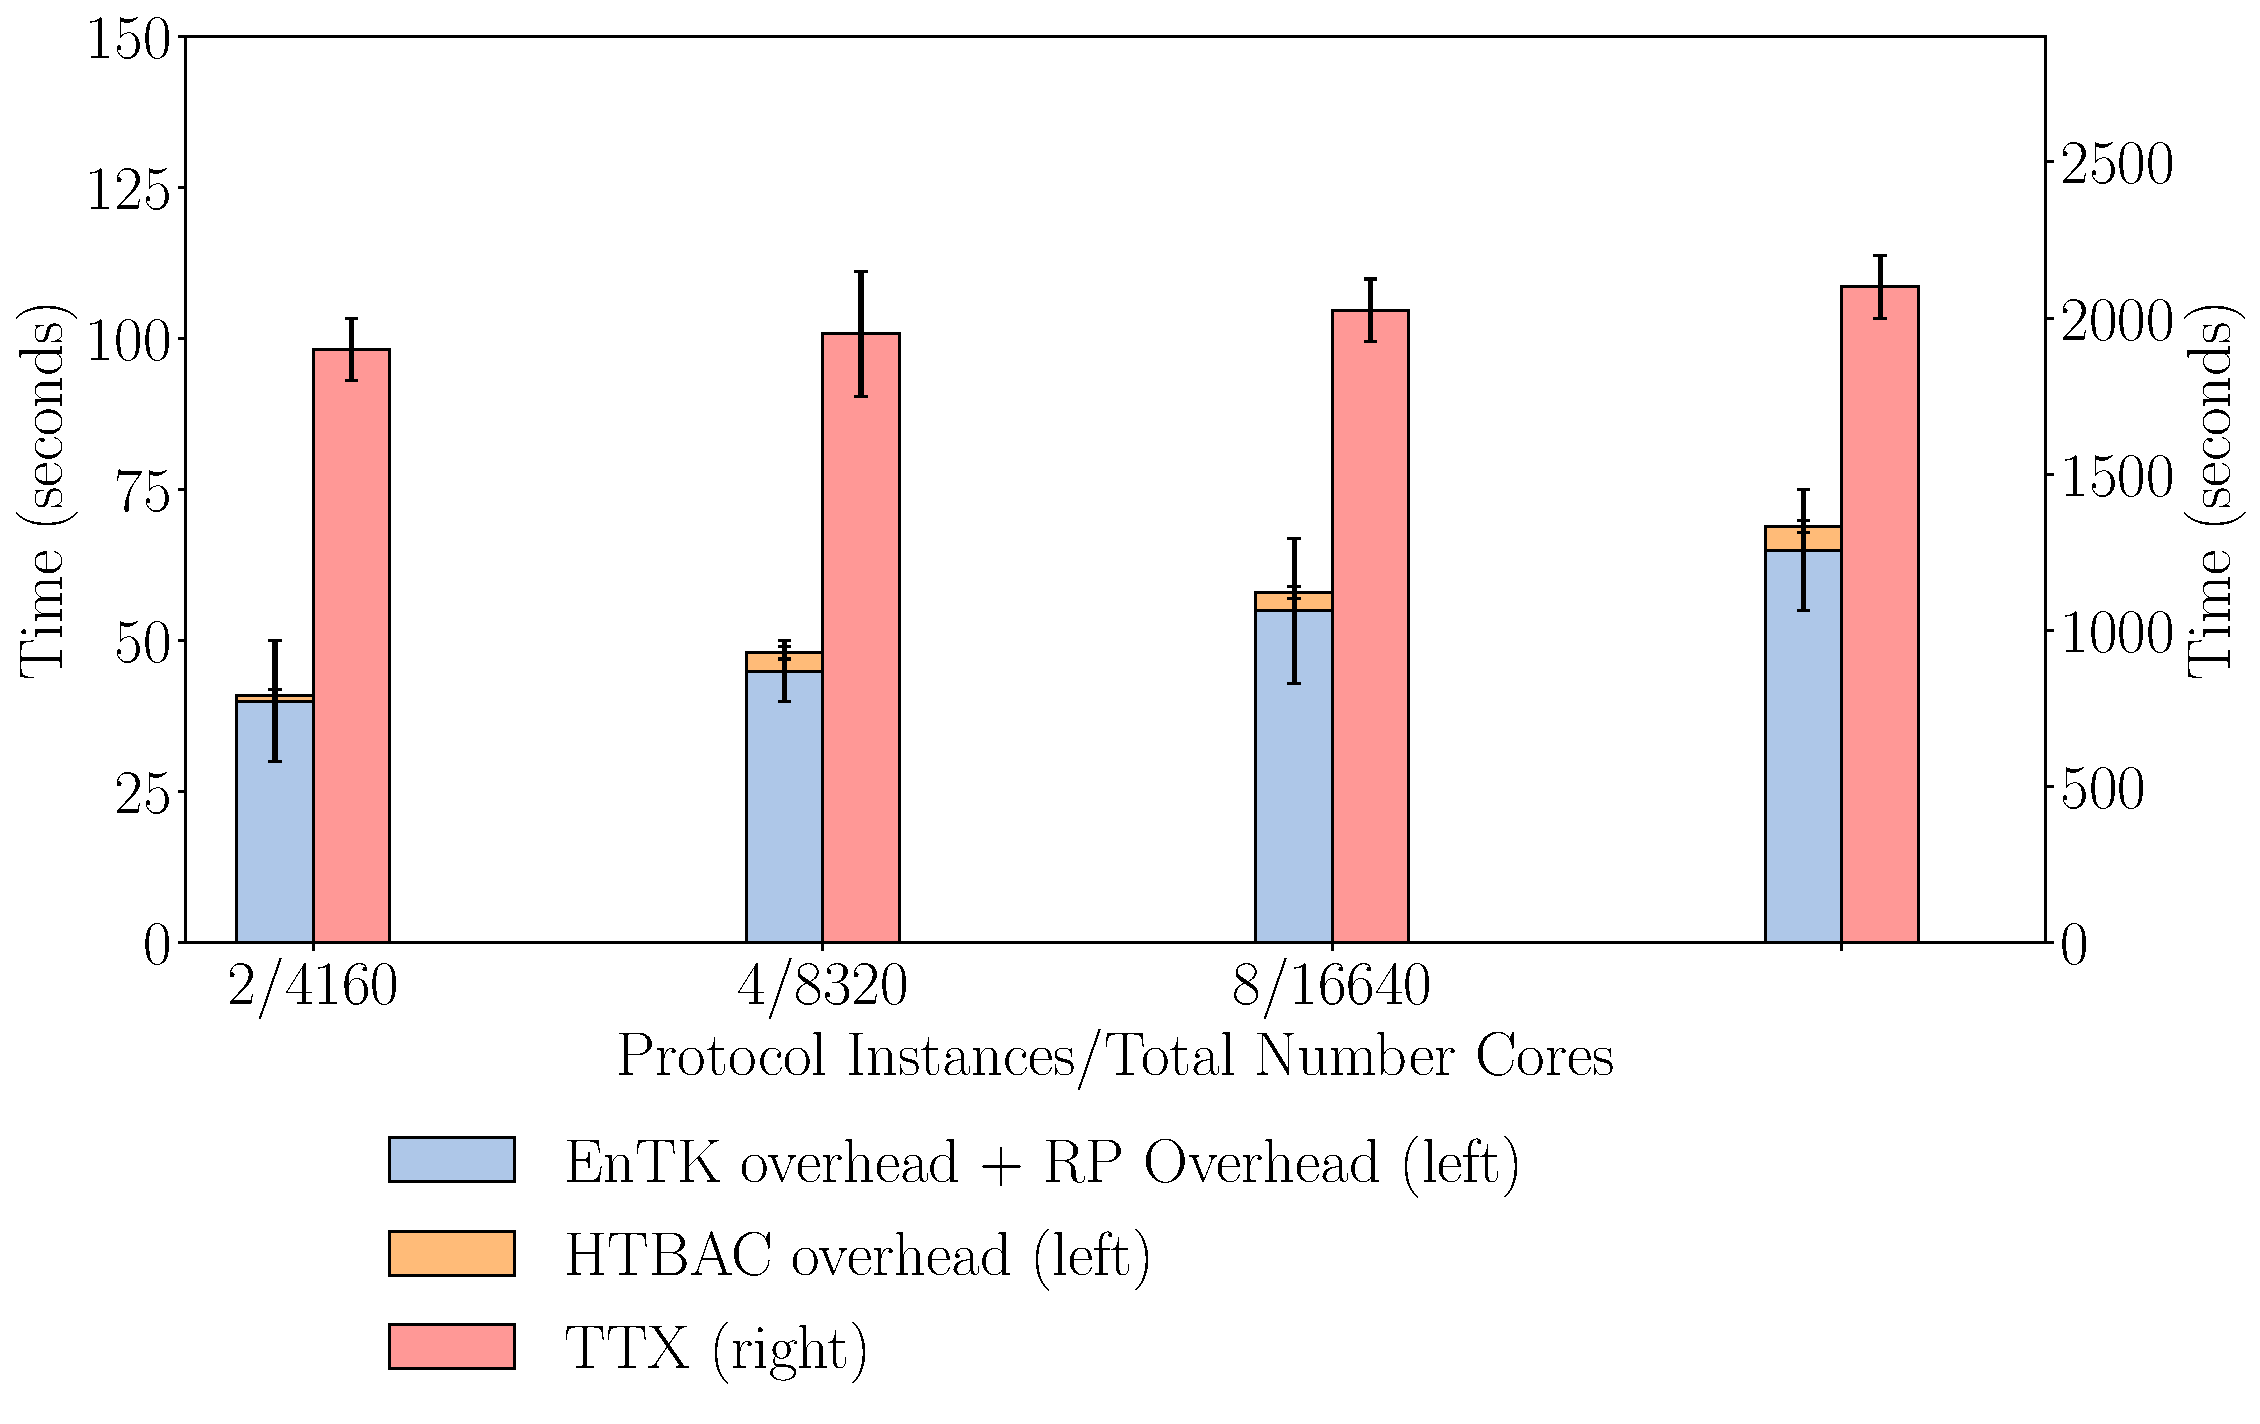
\includegraphics[width=\columnwidth]{figures/new_ws_ties.pdf}
    \caption{Weak scaling properties of HTBAC using TIES protocol. We 
    investigate the weak scaling of HTBAC as the ratio of the number of protocol 
    instances to resources is kept constant. Overheads of HTBAC (right), and 
    runtime overhead (left) and \(TTX\) (left) for experimental configurations
    investigating the weak scaling of TIES. We ran 3 trials for each protocol
    instance configuration.}
\label{fig:weak_scaling_TIES}
\end{figure}

\begin{figure}
  \centering
    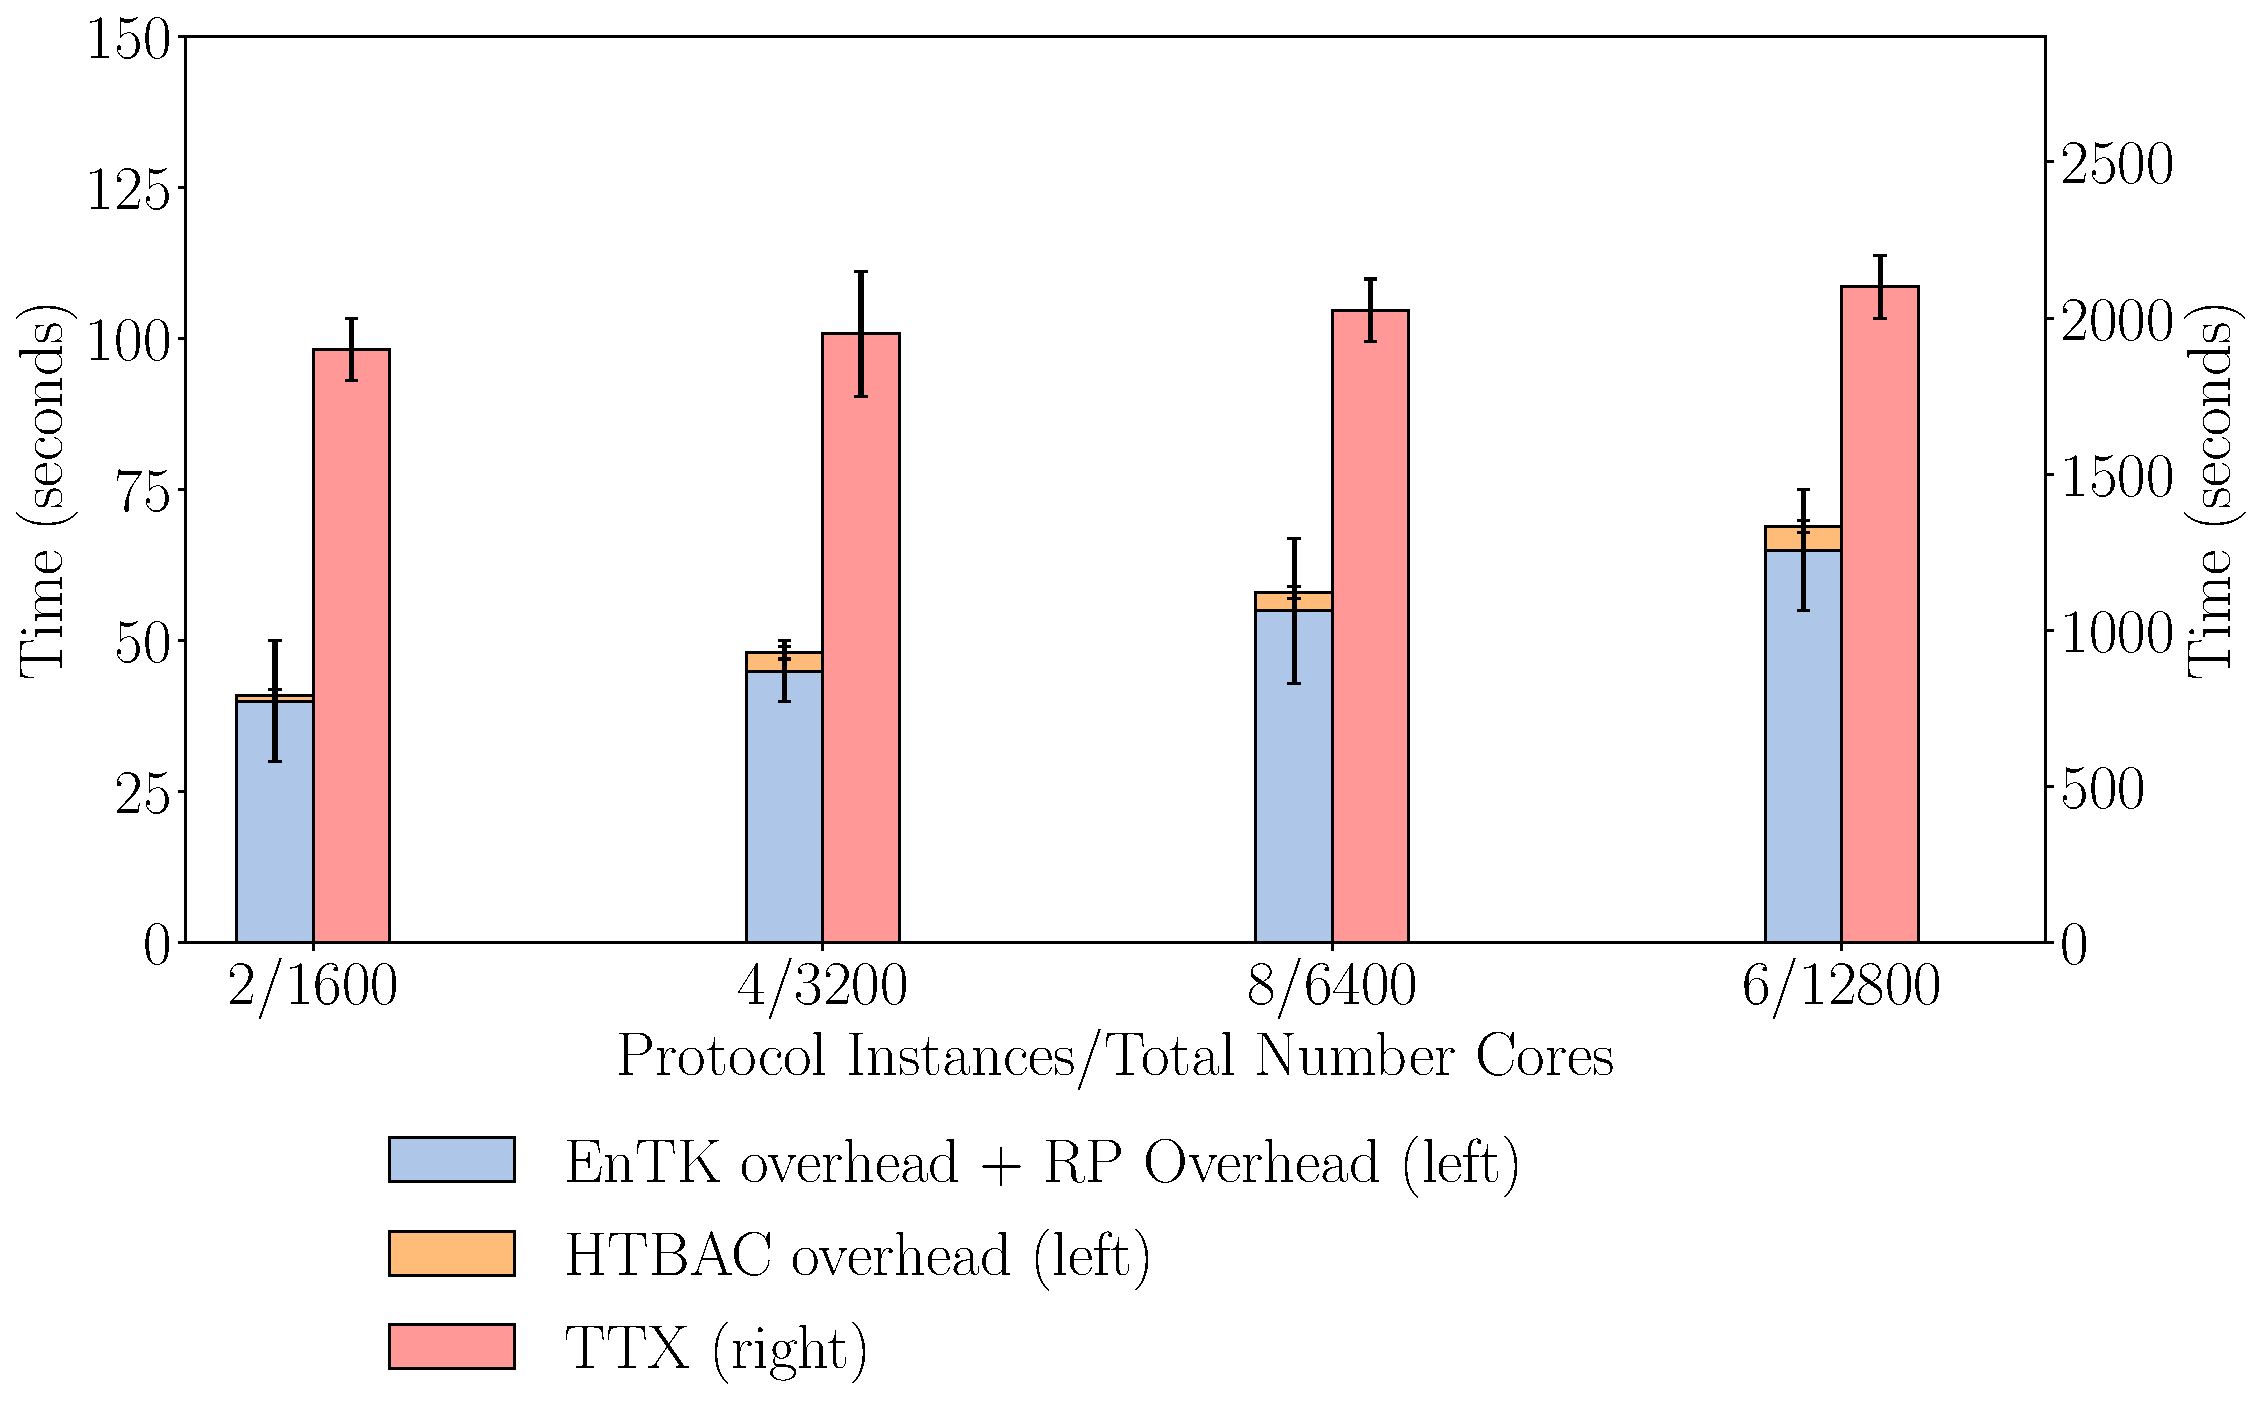
\includegraphics[width=\columnwidth]{figures/new_ws_esmacs.pdf}
    \caption{Weak scaling properties of HTBAC using ESMACS. We investigate the 
    weak scaling of HTBAC as the ratio of the number of protocol instances to
    resources is kept constant. Overheads of HTBAC (right), and runtime
    overhead (left) and \(TTX\) (left) for experimental configurations
    investigating the weak scaling of TIES. We ran 2 trials for each protocol
    instance configuration.}
\label{fig:weak_scaling_ESMACS}
\end{figure}


\begin{figure}
  \centering
    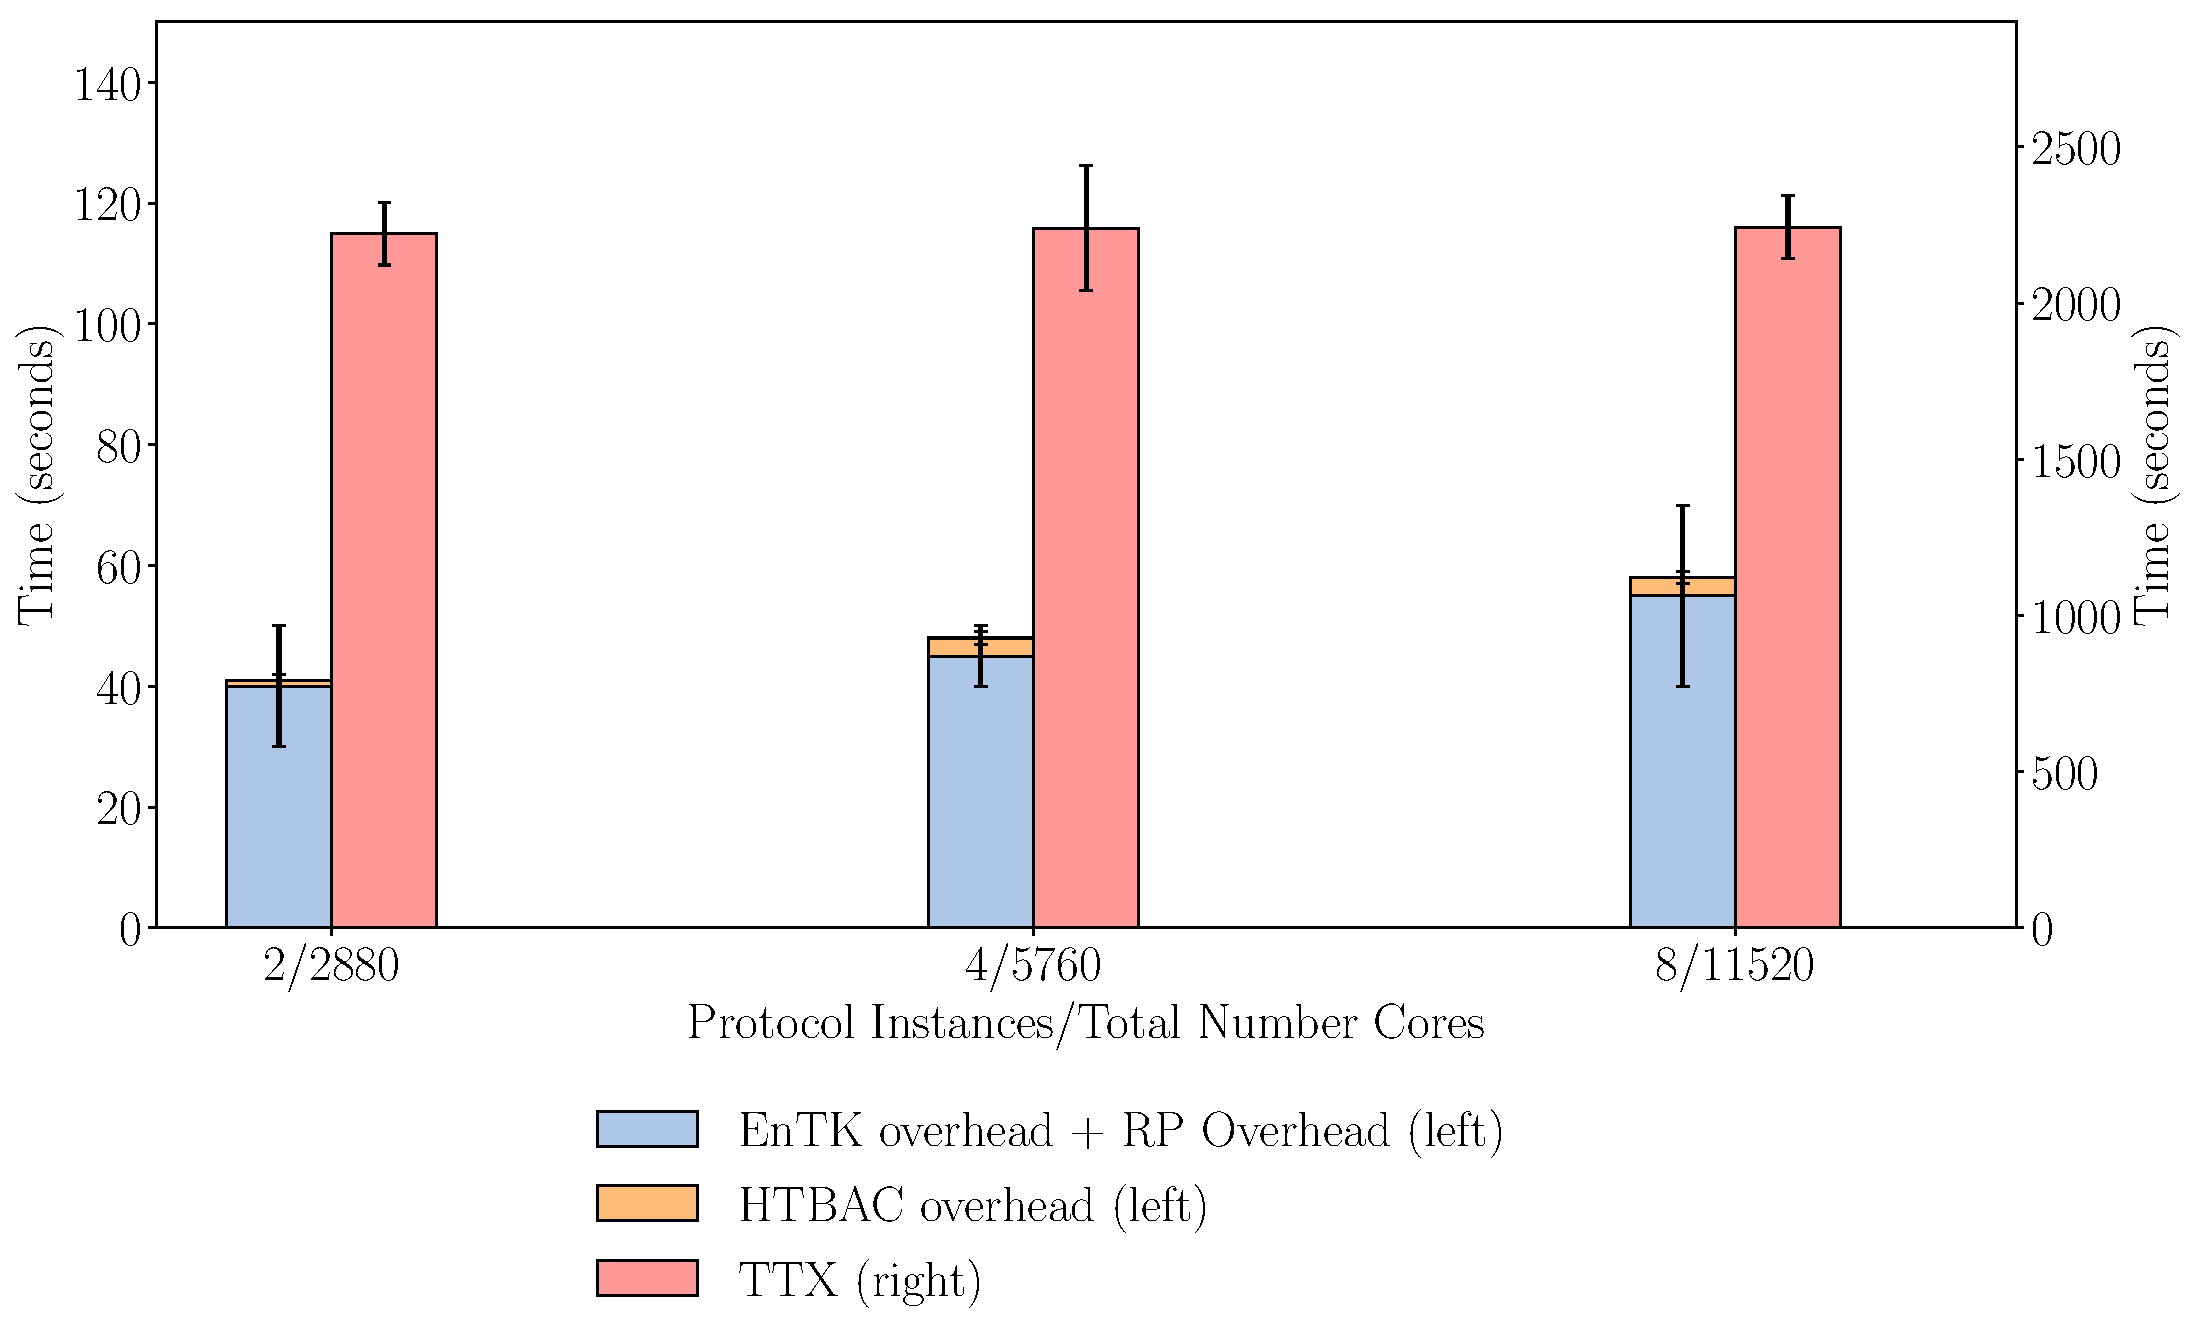
\includegraphics[width=\columnwidth]{figures/new_ws_esmacs_ties.pdf}
    \caption{Weak scaling properties of HTBAC using ESMACS and TIES. We 
    investigate the weak scaling of HTBAC as the ratio of the number of protocol 
    instances to resources is kept constant. Overheads of HTBAC (right), and 
    runtime overhead (left) and \(TTX\) (left) for experimental configurations
    investigating the weak scaling of TIES. We ran 2 trials for each protocol
    instance configuration.}
\label{fig:weak_scaling_ESMACS_TIES}
\end{figure}

\jdnote{Maybe combine captions into 1?}


% ---------------------------------------------------------------------------
\subsubsection{Strong Scaling and Performance Characterization}

\mtnote{Should we have also a `Weak Scaling Experiments' header? Or maybe we
should change this one?}

Next we repeat the same design of the weak scalability experiments but
examine performance of strong scaling when fixing the number of pipelines and
varying the resources. The comparison between weak and strong scalability
shows the overhead introduced by load balancing and scheduling tasks in
multiple generations \mtnote{See previous comments about
terminology}\mtnote{I am not sure I understand: are we comparing overheads
when weak and strong scaling our applications/workflows or are we first
measuring the overheads when strong scaling and then comparing them to those
of weak scaling?}. As we scale the number of generation of concurrent tasks
executions, we half the resources allocated by the pilot \mtnote{this should
be explained in the experiment setup and design}.

\mtnote{General note. Experiments about weak and strong scaling show the
behavior of our software stack with one or more workflows/workloads. The
question these experiments answer to is: Given a workload/workflow, does this
software stack scale weakly and/or strongly? This is why, in the analysis of
our data, we look at the linearity (or lack of thereof) of our plots. The
analysis of the overhead(s) answer to a different question: What part of a
measure---e.g., time to completion---depends on the properties of an element
used to produce that measure---e.g., a component of our software stack?
Usually, the analysis of the overheads is used to explain why we observe lack
of scalability (weak or strong) as represented by a superlinearity in our
plots. The discussion of our experimental results should clearly distinguish
these questions and properly relate the study of scalability to that of
overheads. At the moment, our discussion does not do all this.}

Furthermore, as we scale the number of generations, the runtime overhead of
RP scales linearly. RP requires an amount of time to schedule tasks
proportional to the scale of execution. The main contributor to the increase
in overhead \mtnote{which one?} is derived \mtnote{I am not sure a
contributor is derived} by the time of resources inactivity while RP
schedules new tasks \mtnote{this is derived from another publication: we need
to reference the work we copy/paraphrase from}. As such, the overhead is
expected to grow proportionally to the number of concurrent tasks.

The RP overhead decomposes \mtnote{I do not think the overhead decomposes: Do
we measure the components of the overhead?} into events \mtnote{we use events
to record timestamps from which we derive durations that, once interpreted,
measure our overheads. I would avoid to mention events in this context.} that
capture the pilot and tasks lifespan. The pilot duration contains the time to
bootstrap and terminate the pilot. The task overheads contain the executor's
spawning of the task, folder staging preparation, and operating system task
spawning. \mtnote{We need to explain to the reader why all this is relevant
in this context.} \jdnote{need to discuss on 06/04}

\begin{figure}
  \centering
    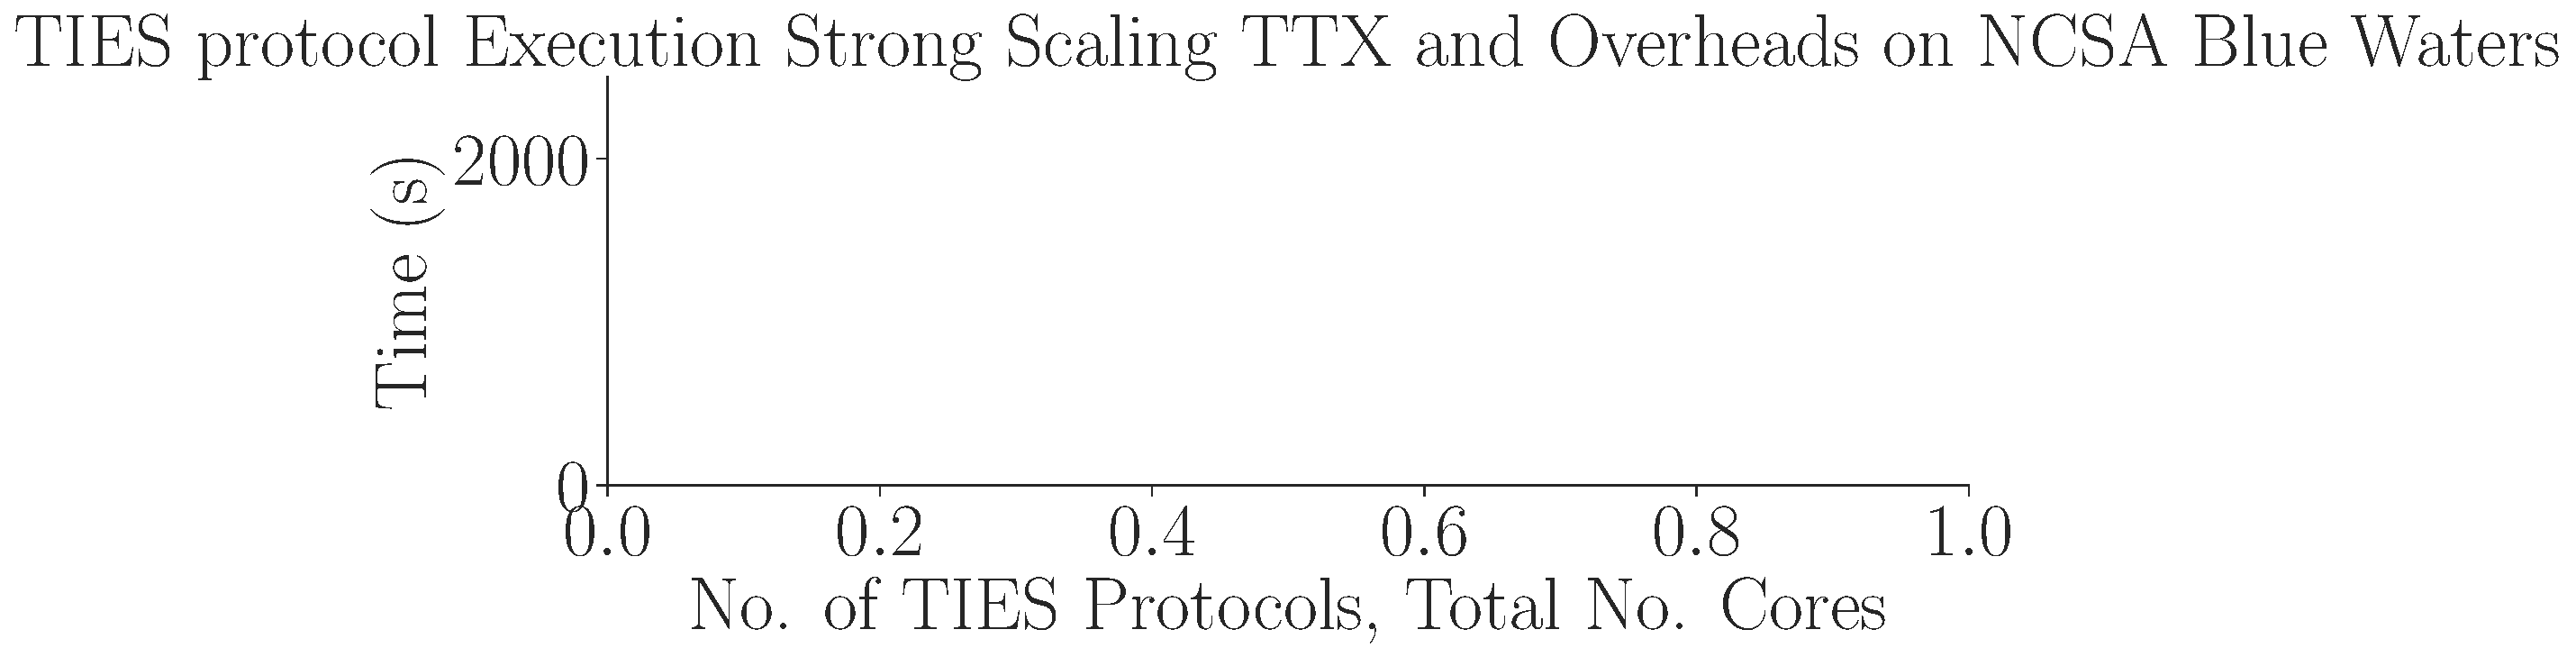
\includegraphics[width=\columnwidth]{figures/ties_ss_pseudo.pdf}
    \caption{Strong scaling properties of HTBAC using TIES protocols. We
    investigate the strong scaling of HTBAC with a fixed number of protocol
    instances while varying the amount resources. Overheads of HTBAC and
    runtime overhead (left) and \(TTX\) (right) for experimental
    configurations investigating the strong scaling of TIES.}
\label{fig:strong_scaling_TIES}
\end{figure}



%----------------------------------------------------------------------------
\subsection{Validation Experiments}

% \mtnote{Validation ExperimentS?}

% HTBAC automates the process of calculating the binding affinity of
% protein-ligand complexes from reading the input to analyzing the final
% results. 

In order to validate the correctness of the results produced using 
HTBAC and the BRD-GSK physical systems, we have devised
a set of experiments. These experiments are vital to gain confidence in the
algorithm and to prove that it is indeed calculating the correct values.

The validation experiments were based on the original study of Wan et. al.
\cite{Wan2017brd4}. We selected a subset of the protein ligand systems that
were the subject of that study: they are the ligand transformations 3 to 1,
4, and 7. We then performed a full simulation on all 3 systems and calculated
the binding affinity (see Table~\ref{tab:exp2}) using HTBAC.

The results show that all three $\Delta \Delta$G values are within error bars
of the original study, reinforcing the fact that HTBAC has indeed correctly
implemented the complex workflow of TIES.

\begin{table}
  \centering
  \caption{Comparison of the calculated binding free energies using HTBAC,
  from the original study by Wan et. al and experimental data. In principle,
  the two theoretical studies used the same protocol. This experiment proved
  that HTBAC implemented TIES correctly, as the calculated values are either
  the same or within error bar of the original study. All values are in
  \textbf{kcal mol\textsuperscript{-1}}.}
  % \begin{tabular}{l@{\hskip 1in}r@{\hskip 0.2in}r@{\hskip 0.2in}r}
  \begin{tabular}{lrrr}
    \toprule
    System & HTBAC & Wan et. al & Experiment \\
    \midrule
    BRD4 \textbf{3 to 1} & \num{0.39 +- 0.10} &   \num{0.41 +- 0.04} &  \num{0.3 +- 0.09} \\
    BRD4 \textbf{3 to 4} & \num{0.02 +- 0.12} &   \num{0.01 +- 0.06} &  \num{0.0 +- 0.13} \\
    BRD4 \textbf{3 to 7} & \num{-0.88 +- 0.17} &  \num{-0.90 +- 0.08} & \num{-1.3 +- 0.11} \\
    \bottomrule
  \end{tabular}
  \label{tab:exp2}
\end{table}

%----------------------------------------------------------------------------
% \subsection{Adaptive Experiments}

% The TIES workflow can benefit from an adaptive execution environment to
% improve the efficiency and accuracy of result. In \emph{adaptive experiments}
% we implemented the adaptive quadrature algorithm specifically customized for
% biosimulations.

% In the adaptive workflow, we alter the number of $\lambda$ windows being
% simulated over the course of a protocol instance. The position of new
% $\lambda$ windows depends on the estimated error of the integral measured
% between adjacent windows. Increasing the number of $\lambda$ windows in
% regions of rapid change will increase the accuracy of the overall integral to
% a greater degree than an arbitrarily placed window. In order to adaptively
% add lambda windows, we need access to the $\partial U/\partial\lambda$ values
% during runtime. Therefore, we break down the single production simulation
% stage (S4) \mtnote{I would reference the figure with the workflow diagram
% here} from the nonadaptive workflow into multiple smaller stages \mtnote{how
% many?}, each running for 1 ns. Once each simulation is complete within a
% stage, a decision is made about whether more $\lambda$ windows are required,
% and, if so, where these windows should be placed.

% We start out the simulation with 5 replicas of \emph{3} \mtnote{why emphasis
% for 3?} equally spaced $\lambda$ windows, and equilibrate them. Then we
% repeatedly execute shorter production simulations followed by an analysis
% phase which determines where to place new lambda windows. This procedure is
% repeated until convergence, at which point all concurrent simulation are
% terminated. We define convergence as the point in the production-analysis
% loop at which a desired error threshold is reached.

% The success of this algorithm is determined by the decision where additional
% $\lambda$ windows should be introduced. In adaptive quadrature, this decision
% is made by calculating an error estimate on the integral and comparing this
% estimate to a threshold value. Due to the stochastic nature of
% biosimulations, it is non-trivial to determine this error and, as a proof of
% concept, we simplified this decision to replicate pre-calculated results. In
% future studies, we plan to use a dynamic decision process.

% Inter-node communication introduces a constraint on the number of new $\lambda$
% windows that can be added at each iteration. Simulations must run on an
% integer number of nodes to reduce the overhead of inter-node communication.
% This means that the number of new $\lambda$ windows (i.e., the number of
% simulations) \emph{has} to be either doubled or left unchanged. If the number
% of windows is doubled, the number of nodes per simulation can be halved
% automatically. Our algorithm loops through the current $\lambda$ window pairs
% until this criterion is reached, forcefully adding more windows when needed.


% % I don't think we need this equation here, it's too trivial.
% % \begin{flalign}
% % L &= \{ x_i: x_i\in[0,1]\; and\; x_{i+1} = x_i + \delta \}, where\ \delta\ is\ 0.5.
% % %&$$L=\{ x_i: x_i\in[0,1]\; and\; x_{i+1} = x_i + \delta \}$$%, where $\delta$ is $0.1$.
% % \end{flalign}

% % For every $\lambda$ window we initialize with five replicas therefore
% % yielding a total of 15 tasks. We run 15 tasks for stages $S1$ through
% % $S4.1$. Between stages $S4.1$ and $S4.3$ the number of $\lambda$ windows
% % doubles for every stage, which doubles the total number of tasks. The last
% % production simulation stage, $S4.4$, runs for the remaining 2 ns durations.

% Our experiments implement adaptive change in the $\lambda$ windows sampled
% and not the timing of execution. In this way, we introduce only a single
% \mtnote{additional?} degree of freedom relative to \mtnote{compared to?} our
% baseline ``non-adaptive" experiments. HTBAC provides the functional
% capability to adaptively determine the time at which the $\lambda$ windows
% are chosen. However, in this paper we do not investigate the impact of such
% adaptivity, as the objective is to determine the feasibility of adaptive
% execution and the scientific merit of adaptive decision making.

% \begin{figure}
%   \centering
%    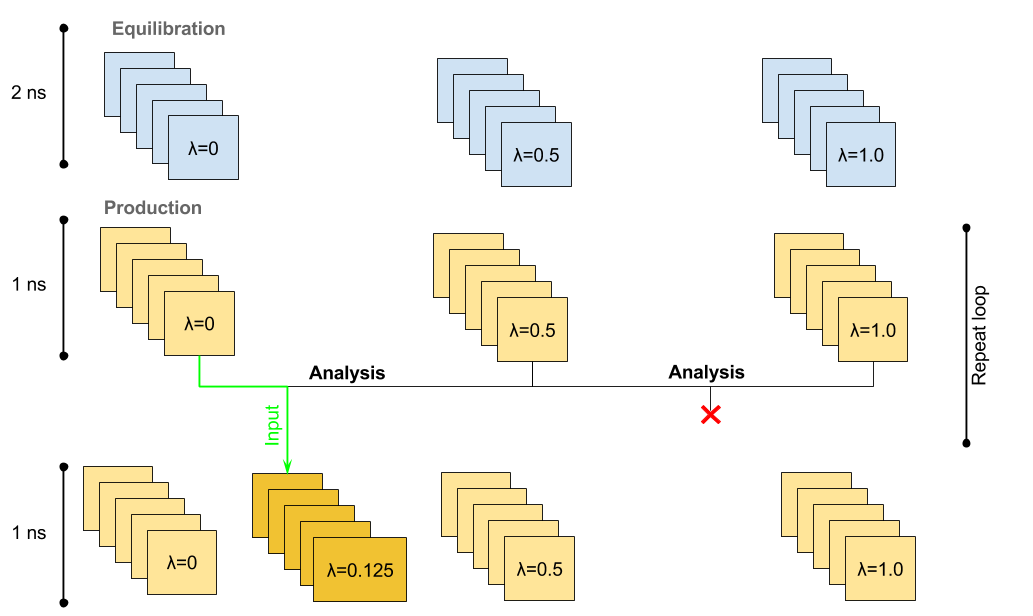
\includegraphics[width=\columnwidth]{figures/Adaptive_TIES_1.png}
%   \caption{Illustrating the adaptive workflow. After the 3 initial lambda 
%   windows are equilibrated, the first production stage starts. 
%   This is followed by analysis at every lambda interval, to decide whether 
%   to add a new window in the middle. The production-analysis is repeated 
%   for 4 production steps in our implementation, not shown here.}
% \label{fig:adaptive_TIES}
% \end{figure}

%----------------------------------------------------------------------------


\begin{figure}
  \centering
    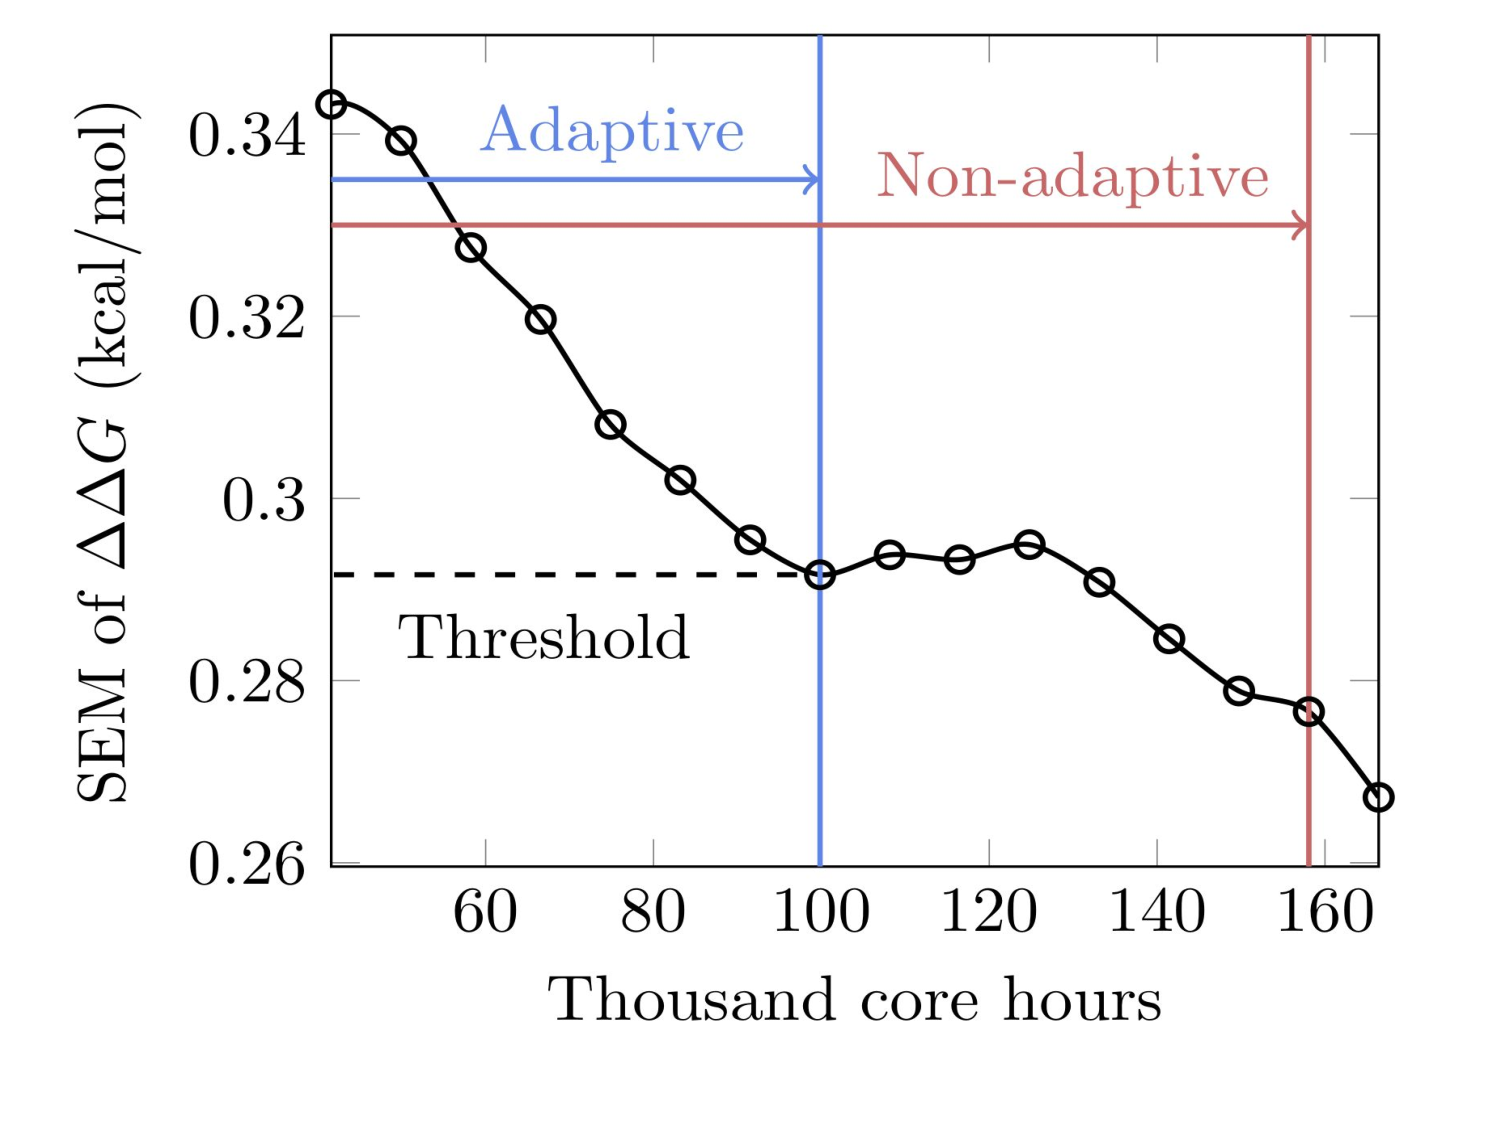
\includegraphics[width=\columnwidth]{figures/adaptive_vs_nonadaptive_pseudo.pdf}
    \caption{Illustrating the adaptive vs. non-adaptive workflow given the
    same number of core hours}
\label{fig:adaptive_vs_nonadaptive_TIES}
\end{figure}

% ---------------------------------------------------------------------------
\subsubsection{Adaptive Quadrature Experiments Results}

\mtnote{Should this be Results as a whole? Or are we missing the results for
all the others?} \kfnote{I think results and experiments are one section. 
This subsubsection is for the adaptive quadrature. There is a separate one for 
adaptive termination.}

The aim of introducing adaptive quadrature to alchemical free energy 
calculation protocols (e.g. TIES) is to reduce time to completion while 
maintaining (or increasing) the accuracy of the results. Time to completion is 
measured by the number of core hours consumed by the simulations. Accuracy is 
defined as the error with respect to a reference value, calculated via a dense 
lambda window spacing (65 windows). This reference value is used to establish 
the accuracy of the non-adaptive protocol (which has 13 lambda windows) and the 
adaptive protocol (which has a variable number of lambda window, determined at 
run time).

One of the input parameters of the adaptive quadrature algorithm is the desired 
error threshold that the estimated integral should be below of. We set this 
threshold to the error of the non-adaptive algorithm calculated via the 
reference value. The algorithm then tries to minimize the number of lambda 
windows constrained by the accuracy requirement. Table~\ref{tab:adapquad} shows 
the results of running adaptive quadrature on 5 protein ligand systems, 
comparing the time to completion and accuracy versus the non-adaptive case. The 
number of lambda windows are reduced on average by \SI{32}{\percent}, hence reducing the time to completion by the same amount. The error on the adaptive results is also decreased, on average by \SI{77}{\percent}. In the case of the TYK2 L7-L8 system, the non-adaptive error was very low, hence the algorithm had to use a large number of windows to match that accuracy. In fact, by using 1 more window it was able to increase accuracy by \SI{40}{\percent}. 

\begin{table*}
  \caption{Comparing results of adaptive, non-adaptive and reference runs}
  \label{tab:adapquad}
  \begin{tabular}{lSSSSSS}
    \toprule
    {System}                               & 
    {Ref $\Delta \Delta$G}                 &
    {Non-adaptive $\Delta \Delta$G}        &
    {Adaptive $\Delta \Delta$G}            &
    {Num. of $\lambda$ windows}            &
    {Decrease in time to completion}       &
    {Increase in accuracy}                 \\
    \midrule
    {PTP1B L1-L2}   & 
    -58.51 & 
    -57.87(64) & 
    -58.60(9) & 
    10 & 
    \SI{23}{\percent} & 
    \SI{86}{\percent} \\
    %
    {PTP1B L10-L12} & 
    1.83   & 
    2.05(22) & 
    1.94(7)  & 
    6  & 
    \SI{54}{\percent} &
    \SI{68}{\percent} \\
    %
    {MCL1  L32-L38} & 
    2.13   & 
    2.33(20) & 
    2.14(1)      & 
    7  & 
    \SI{46}{\percent} & 
    \SI{95}{\percent} \\
    %
    {TYK2  L4-L9}   &
    -28.69 & 
    -28.25(44) & 
    -28.67(1)  & 
    7  & 
    \SI{46}{\percent} & 
    \SI{98}{\percent} \\
    %
    {TYK2  L7-L8}   & 
    4.97   & 
    4.92(5) & 
    5.00(3)      & 
    14 &  
    \SI{-8}{\percent} & 
    \SI{40}{\percent} \\
    \bottomrule 
    
  \end{tabular}
\end{table*}

Figure~\ref{fig:adapquad} shows progression of the algorithm, starting from the 
3 initial lambda windows, and at each iteration bisecting the interval where 
the error is above the set threshold. For system X, we can see as how the parts 
of the function that change less have relatively fewer windows, while parts of 
greater change (usually, though not always around the $\lambda=0.5$ mark) have 
more lambda windows to capture the function shape better. 

\kfnote{Move this to algorithm description} In previous studies \cite{} the 
error estimation during the adaptive algorithm is done via calculating the 
integral estimate via two methods, one lower and one higher in complexity, then 
the difference between the two can constitute as a rough estimate of the error 
on that interval.


One way to visualize the adaptivity in this experiment is to plot the
function and integral approximations at every iteration.
Figure~\ref{fig:adapt} shows how the value of $\Delta$G (i.e., the integral
of the function) for test system \textbf{3 to 7} \mtnote{I would not mix
different formats of emphasis: should we use only emph?} improves as the
algorithm places more lambda windows. It is important to note that the new
points are decided {\it a priori} for reasons discussed above but this is
opaque to the algorithm. This shows we have initial adaptive capabilities,
paving the way to more advanced biosimulation algorithms.

\begin{figure}
  \centering
\begin{tikzpicture}
\begin{axis}[
  xlabel=$\lambda$,
  ylabel=$\frac{dU}{d\lambda}$,
  xmin=0,
  xmax=1,
  legend pos=north west,
  grid=both,
  ]
  \addplot+[name path=alch_1, mark size=1pt, mark=*, color=blue] table [x=lambda, y=p1v]{alch_1.csv};
  \addlegendentry{Iteration 1: Initial};

  \addplot+[name path=alch_2, mark size=1pt, mark=*, color=red] table [x=lambda, y=p1v]{alch_2.csv};
  \addlegendentry{Iteration 2: Increase};

  \addplot+[name path=alch_3, mark size=1pt, mark=*, color=brown] table [x=lambda, y=p1v]{alch_3.csv};
  \addlegendentry{Iteration 3: Optimized};

  \addplot+[name path=alch_4, mark size=1pt, mark=*, color=black] table [x=lambda, y=p1v]{alch_4.csv};
  \addlegendentry{Iteration 4: Sampling};

  \addplot[name path=line, draw=none] {0};

  \addplot fill between[
    of = alch_1 and line,
    split,
    every even segment/.style = {pattern color=blue!50, pattern=vertical lines},
    every odd segment/.style = {pattern color=blue!50, pattern=vertical lines},
    soft clip={domain=0:1},
  ];

  \addplot fill between[
    of = alch_2 and line,
    split,
    every even segment/.style = {pattern color=red!50, pattern=horizontal lines},
    every odd segment/.style = {pattern color=red!50, pattern=horizontal lines},
    soft clip={domain=0:1},
  ];

  \addplot fill between[
    of = alch_3 and line,
    split,
    every even segment/.style = {pattern color=brown!50, pattern=north east lines},
    every odd segment/.style = {pattern color=brown!50, pattern=north east lines},
    soft clip={domain=0:1},
  ];

\end{axis}
\end{tikzpicture}
\caption{Approximating the intergral under the curve, hence calculating
$\Delta$G. The adaptive algorithm reevaluates the efficiency of the lambda
window mesh after every \SI{1}{\nano\second} and makes a decision whether to
place more lambda windows inside certain ranges. As we iterate every 1 ns,
the integral approximation becomes more accurate.}
\label{fig:adapt}
\end{figure}
